%% wlkr
\documentclass[12pt,journal,compsoc]{IEEEtran}
\usepackage[hidelinks]{hyperref}
\usepackage{graphicx}
\usepackage{float}
\usepackage{listings}

\begin{document}
\title{Final Project}

\author{Ryan Walker, Jin Seo}

\IEEEtitleabstractindextext{%
% \begin{abstract}
% This paper will outline events of the failed Ariane 5 maiden launch. In addition it will describe the failure mode and recommend alternative system design and practices that would have prevented the crash.
% \end{abstract}
}

% make the title area
\maketitle
\IEEEpeerreviewmaketitle

\section{Introduction}
\IEEEPARstart{R}{ecent} advancements in drones have made brushless DC motors (BLDC motors) very inexpensive and lightweight. This has sparked vivid open source development of various motor drivers [\ref{odrive}] and mechanical support components [\ref{opentorque}]. By leveraging these tools we are aiming to build a lightweight 6-axis compliant robot manipulator. In the essence of time, only 3 axis' will be developed and dummy mass will be placed on the end. The following metrics define success for the device.

\begin{center}
\begin{tabular}{ c|c } 
 Spec & Quantity  \\ 
 \hline
 Payload & 1kg \\ 
 Working Area & ? \\ 
 DOF & 3 \\ 
 Speed & ?  \\ 
 Cost & sub \$3k  \\ 
\end{tabular}
\end{center}

\subsection{Motion Control}
\label{odrive}
For the motion control we want something that is open source, can deliver high current and is closed loop. The ODrive ticks all these boxes and more. Thanks to the hard work of developers across the world we have the tools to design powerful electromechancs the can be used to solve real problems. The Odrive is capable of driving two motors and receiving two channels of encoder feedback. We will need to use 3 boards for the entire robot. This comes to a total cost of only 380\$.
  
\begin{figure}[H]
\centering
\caption{ODrive}
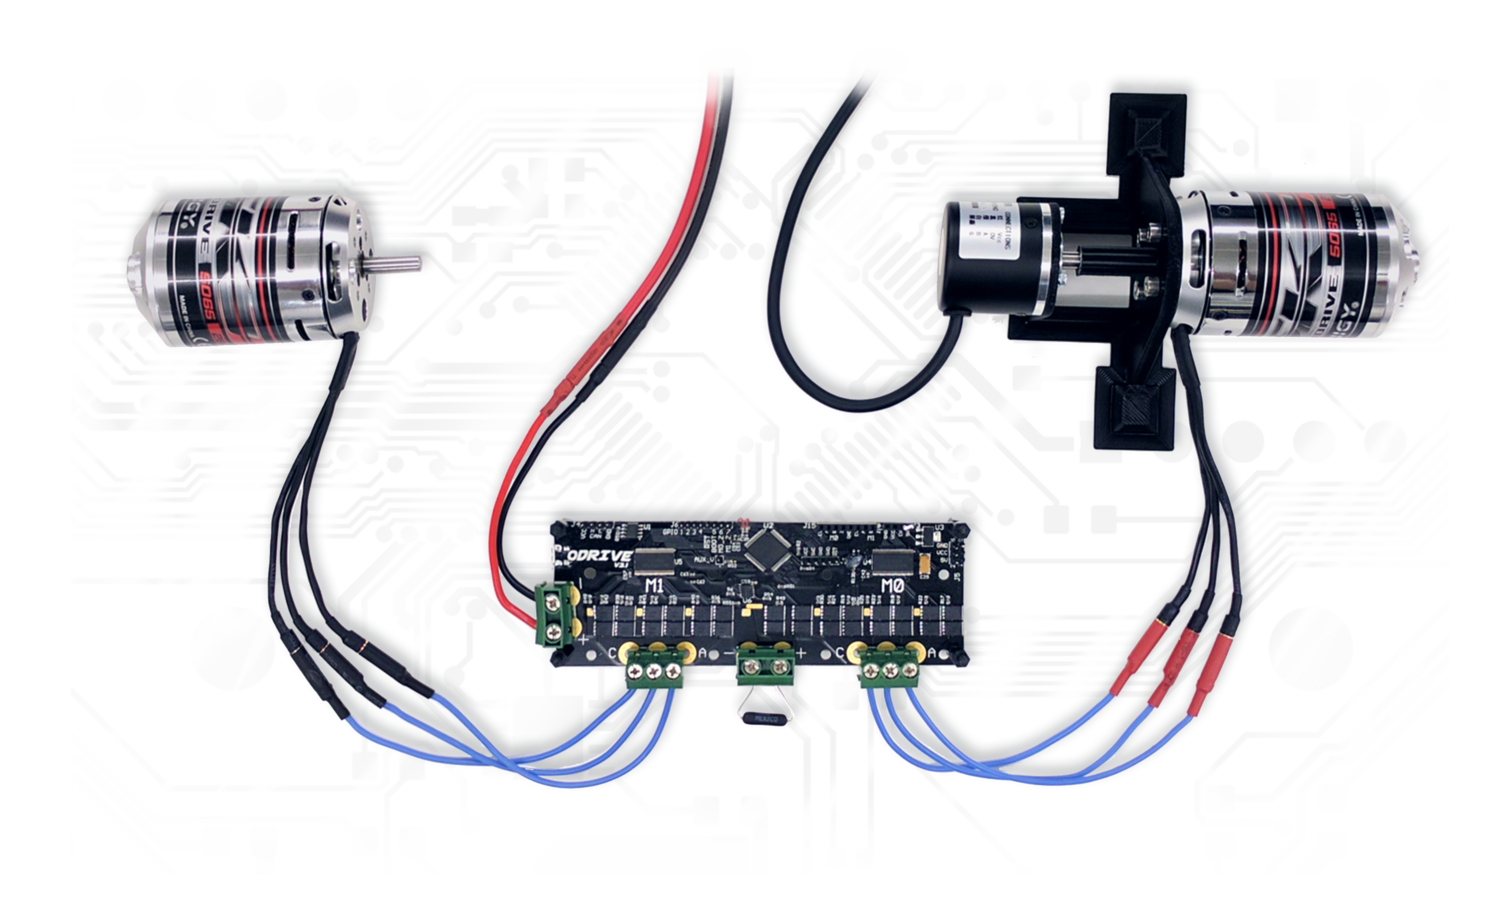
\includegraphics[scale=0.15]{images/odrive.png}
\end{figure}

The firmware is completely open source and will need to be modifies as we require CAN for communication.

\subsection{Motors}
The ubiquity of drones has reduced the cost of motors significantly. The Multistar 9235-100KV has been measured to deliver 4.7Nm \cite{9235T} without a gearbox. It comes at a mere cost of 89\$. 

\begin{figure}[H]
\centering
\caption{9235-100KV}
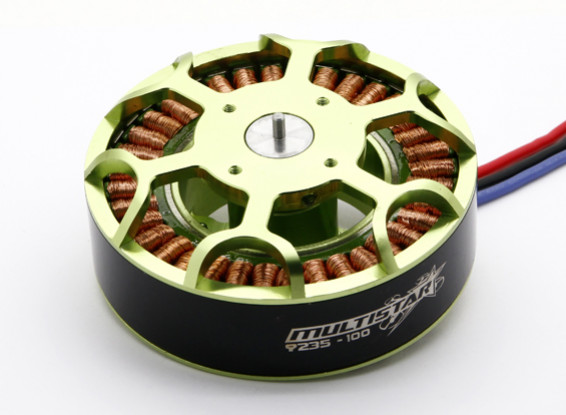
\includegraphics[scale=0.55]{images/motor.jpg}
\end{figure}

\subsection{Gearbox}
OpenTorque is a powerful, compliant actuator for legged robotics. We planning on using it for our revolute robot arm. As each linkage in this style of robot takes away from the payload of the robot, 3d printing something like this out of nylon comes with a serious weight advantage.

\begin{figure}[H]
\centering
\caption{OpenTorque}
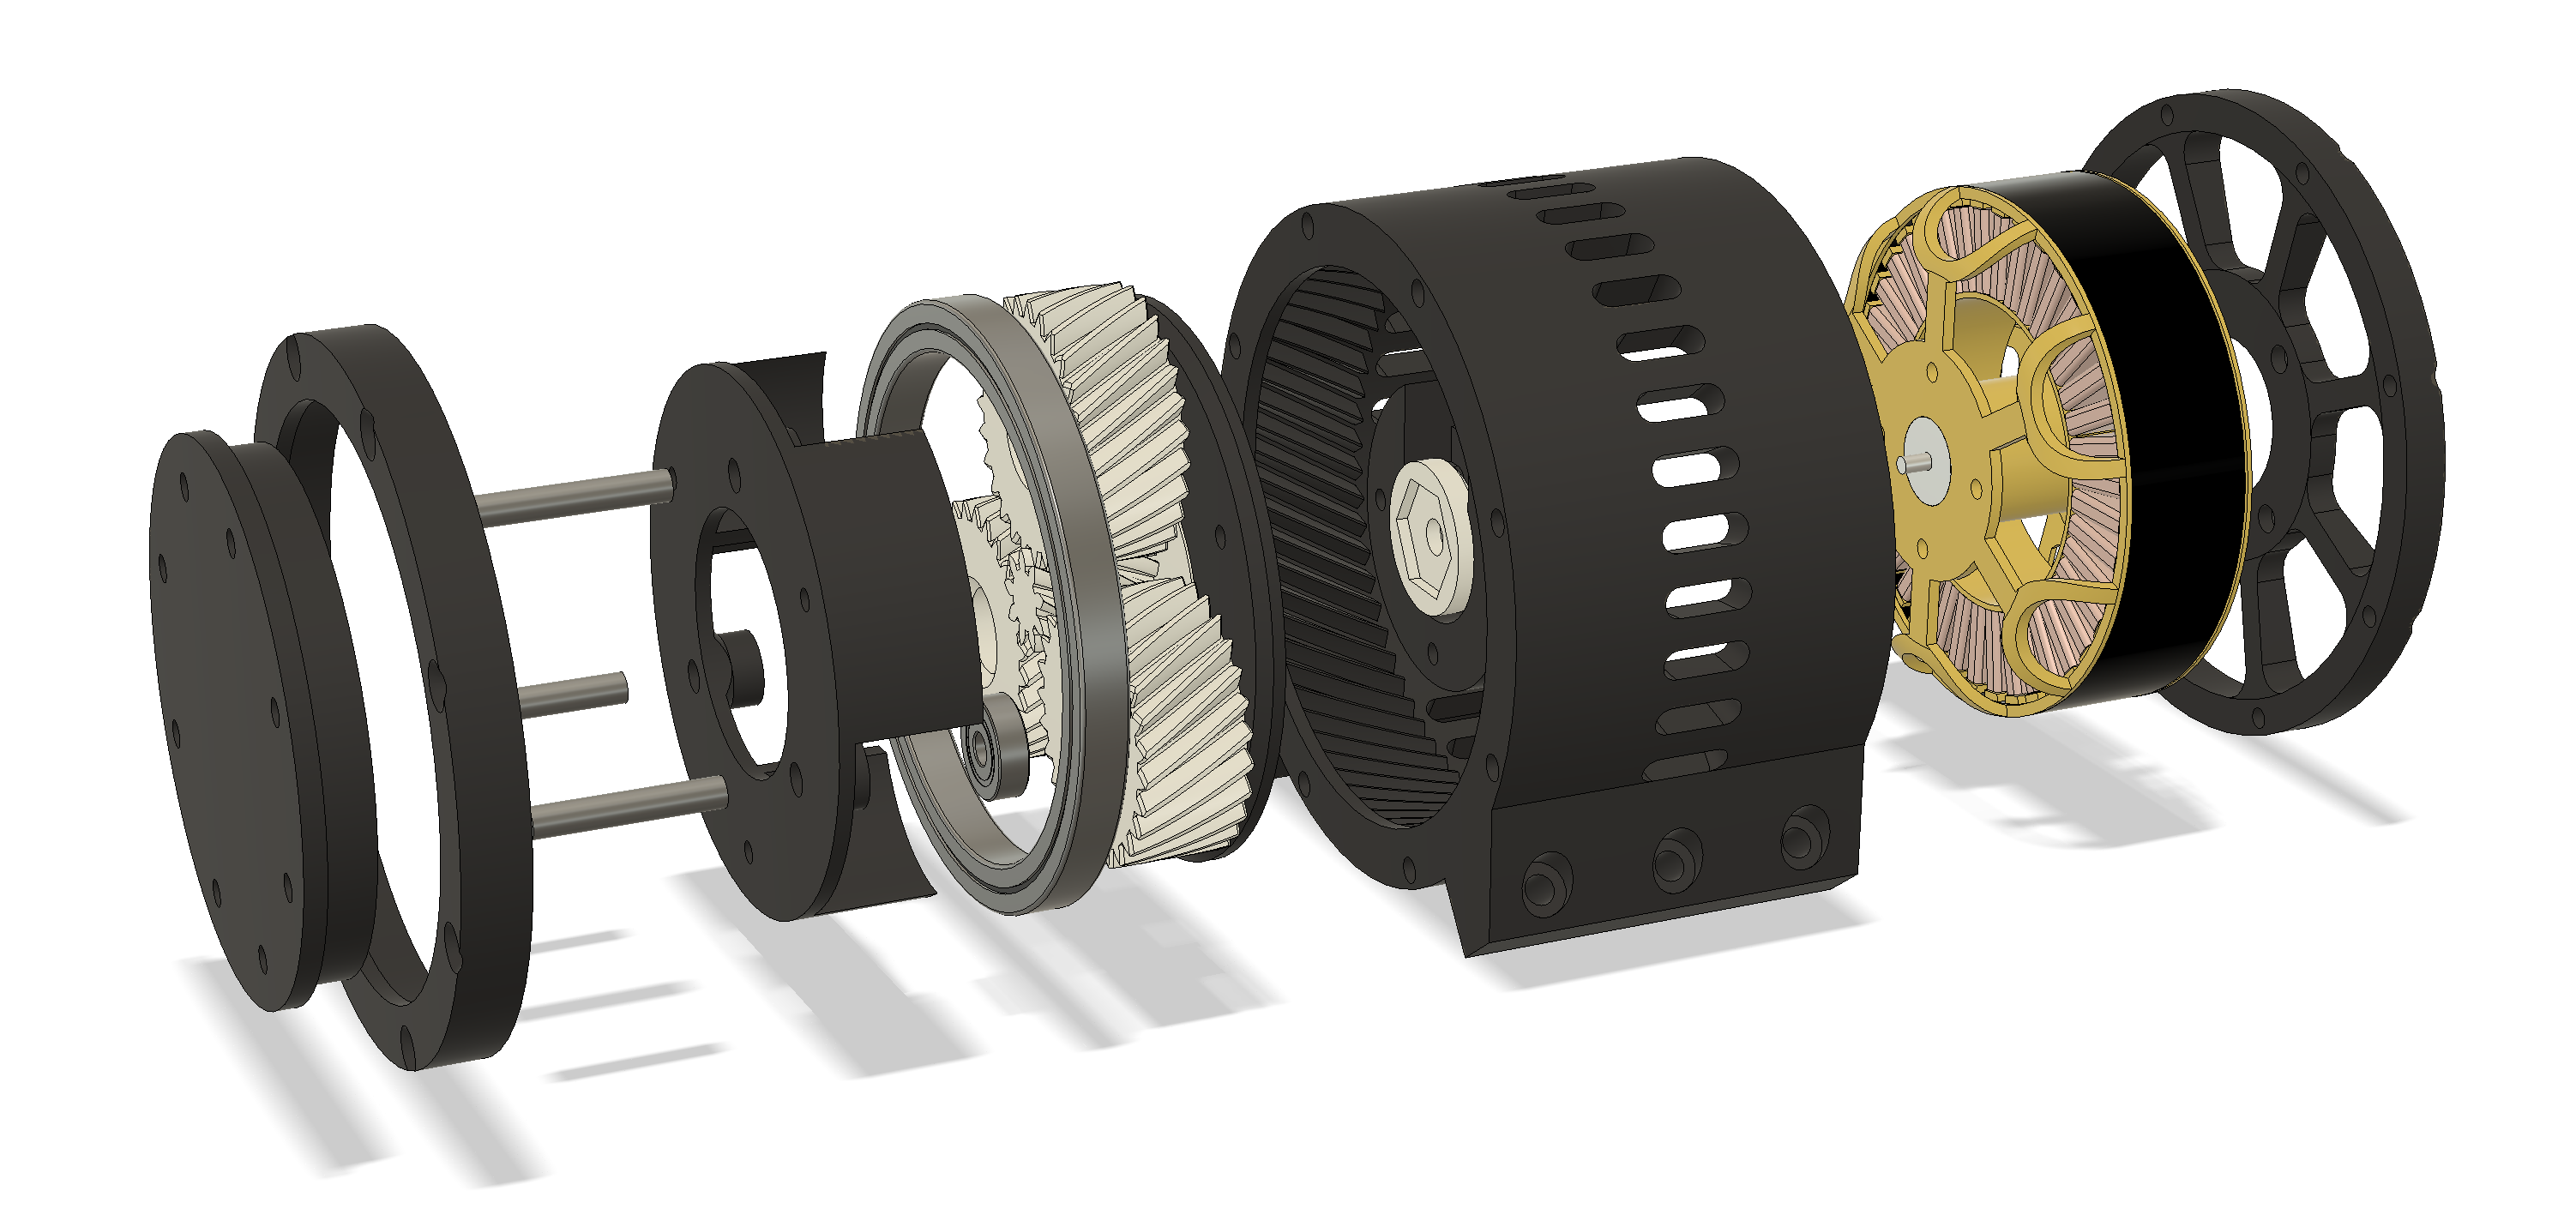
\includegraphics[scale=0.15]{images/openTorque.png}
\end{figure}

% Bib
\begin{thebibliography}{1}
\bibitem{9235T}
Torque measurements for various motors. 
\url{https://docs.google.com/spreadsheets/d/12vzz7XVEK6YNIOqH0jAz51F5VUpc-lJEs3mmkWP1H4Y/edit#gid=0}

\end{thebibliography}


\end{document}

The SRI has been operating on the Ariane 4 without failure for several launches. However, the horizontal velocity of the Ariane 5 is much higher than that of the Ariane 4. This caused an unexpectedly high value of an internal alignment function (BH routine), leading to a software exception. This exception was due to a failed number conversion: The code did an unprotected number conversion from a 64bit float to a 16bit signed integer. Since the float had a greater value than what could fit into the int, this caused a fatal error and the loss of 0.5 billion dollars. \\

The result of the BH function was not needed after liftoff, however the function continued to run for 40 seconds after liftoff occurred. This feature is based on a requirement for the Ariane 4, but is not necessary for the Ariane 5.\\

During the analyses of the software running on the embedded computer, it was found that seven variables were at risk of overflow \cite{501}. However, only four of these variables were protected. This was done because the unprotected variables were believed to be at either a physical limit or have a large margin of safety, which was clearly not the case. In addition a maximum workload of 80\% was set for the SRI computer.

\section{Fault Prevention}
% Burns Page 106, should this be Burns? Or Anderson and Lee?
Burns \cite{BURNS} stated that fault prevention is attempting to eliminate bugs before the system goes live. This can be done using the compiler, software testing, hardware testing and simulations.

\subsection{Code Maintenance}
The rocket was not even using the BH routine during the disaster. It was legacy code that was left in from the Ariane 4. This should have been caught during the design review and removed. This sufferers from the ``if it ain't broken don't fix it'' fallacy. In software design there can be plenty of code that ``ain't broken'', however when the entire system changes you can't just assume that everything will be fine. The running of the BH routine is contradictory to the 80\% workload excuse listed in Section \ref{fail}, if the team was so strapped for resources then why did they have useless code running for 40 seconds after launch? If this code had been removed the failure would not have occurred. 


\subsection{Data Types}
\label{SD}
Without being able to find any schematics of the system I'm making the assumption that there was a 16bit databus which connected the SRI to the onboard computer. The SRI did the float conversion and then put the 16bit number on to the data bus.\\

It's a common misconception that floating point numbers are more precise than fixed point integers. This is not the case, floating point number offer more range. Which was the root of the problem, the number was too big. There are many arguments around ``protecting the conversion''. Protection of the conversion would have prevented the exception, however you still need to \textbf{fit} the number into a 16bit space if you're planning on doing a calculation with it. Just maxing the number could cause havoc with the control system\\

If the programmers did not need the precision of a 16bit int, then they should have put in into a 16bit float. This offers a max number of $\pm65504$, rather then the $\pm32768$ a signed int can take. Doing so would give a $2\times$ margin of error over the int. In addition the conversion should have been protected.

\begin{figure}[H]
\centering
\caption{16bit Float, source: \url{https://en.wikipedia.org/wiki/Half-precision_floating-point_format}}
\label{16}
\includegraphics{16b.png}
\end{figure}

However this technique will take a hit on the precision of the number and requires some conversion time. Another option is to remove an order of magnitude from the 16bit int, this would give more range and less precision as well. Without requiring the extra conversion time. It's up to the designer to decide if these are acceptable trade offs. \\

\subsection{Testing}
\label{testing}
The 501 report \cite{501} lists "There is no evidence that any trajectory data were used to analyse the behaviour of the unprotected variables, and it is even more important to note that it was jointly agreed not to include the Ariane 5 trajectory data in the SRI requirements and specification." \\

This decision wasn't the cause of the failure, however testing like this would have prevented it. The last step in designing a Full Fault Tolerant system is extensive testing. The telemetry data for the rocket could have been numerically calculated and fed into the system. The bug would have made itself obvious and the disaster would have been prevented. Burns \cite{BURNS} calls this fault removal and is a major component of fault prevention.

\section{Fault Tolerance}
% Burns Page 106, should this be Burns? Or Anderson and Lee?
Burns \cite{BURNS} stated that fault tolerance is  the ability for your system to keep running in the presence of faults. This is very challenging in embedded system as there typically can't be any human interaction. However when the hardware inevitably fails there should be routines to handle this. \\

% The Ariane 5 would have to be ``Full Fault Tolerant'', meaning that in the event of a fault then ship needs to keep flying.

\subsection{Redundancy}
\label{Red}
Redundant hardware is used extensively in Full Fault Tolerant system. Redundancy provides alternative hardware in the event of a failure of the main hardware. Burns \cite{BURNS} wrote about Triple Modular Redundant (TMR) systems where three identical pieces of hardware are running in parallel. If the output of one is too far off then the others, it's result is masked out in the computation. This same idea can be extended to $N$ pieces of hardware\\

The Ariane 5 had two parallel SRI systems running. This means that in the event of a sensor or CPU hardware failure it was possible to switch out to the backup SRI. However the failure was not a hardware failure, it was a software failure. So both the main and redundant systems failed from the same software failure. Therefore redundancy did not save the Ariane 5.\\

Burns \cite{BURNS} spoke of the software equivalent to TMR, so called ``$N$-version'' programming. This is a method of software design which which requires $N$-groups of software developers to develop their own codebase, without interaction with each other. The software is then run in parallel and takes the same form as TMR. \\

However Burns listed three major issues with $N$-Version Programming:

\begin{enumerate}
\item Poor Initial Specification
\item Lack of Independence of Design Effort
\item Inadequate Budget
\end{enumerate}

Sections \ref{testing} and \ref{execpt} outlined some serious issues with the initial spec, an implementation of $N$-Version programming would have suffered. The control system for the Ariane 5 is a complex system, so it would be challenging to prevent people from sharing resources and ideas. Finally, would three independent development paths be affordable? Typically the most expensive resource of an embeded system is the development time, I don't think it would be reasonable to $3\times$ this.\\ 

$N-Version$ Programming is a novel approach to the problem and could have been used to avoid the disaster, however the feasibility is still a question. I would recommend approaching the problem  

\subsection{Exception Handling}
\label{execpt}
The specification for the design stated that during an event of a software exception, the system should indicate the failure on the databus to be stored in EEPROM memory. This is followed by a processor shutdown. This technique seems reasonable in three situations:
\begin{enumerate}
\item Debugging environment.
\item System with ``N-Version Programming'' where the OBC would detect the exception and another system can take over. (See Section \ref{Red}).
\item System that catches the exception and can self correct. 
\end{enumerate}
This technique in not reasonable for a system that has no backup routine for exceptions. The OBC read the software exception bitstream and interpreted as data. As the BH routines wasn't even being used at this time of the crash, ignoring the software exception would have been a better response and would have saved the rocket.\\

A somewhat reasonable approach would be to have understood that there was an exception on the databus and extrapolate data. This would be an absolute fallback routine that is still very non-ideal, but better than what was implemented.

\subsection{Conversion Protection}
Baber \cite{SW} has spoken vividly about the conversion. I've written some code below to demonstrate a possible solution that would offer the protection. 

\input{$HOME/wlkrUtils/TeX/codeCBW.tex} %For C
\lstinputlisting{../conv.c}
After examining the code the flaw becomes obvious, is the event of an overflow the max number will be presented. It's possible to make range and precision trade offs, which is discussed more rigorously in Section \ref{SD}. If it's not possible to make these trade offs then a simple handshaking routine could be implemented, this is shown in Section \ref{Nconv}\\


\subsection{Handshaking For Conversion}
It's entirely possible that the team had the processing overhead to implement a handshaking protocol, shown below. 
\label{Nconv}
\lstinputlisting{../convN.c}
This is using a special bit pattern to indicate to the embedded computer that the incoming data will not be a 16bit integer, but a 32 bit integer. In addition code should be implemented to ensure that the 64bit number isn't higher than what can fit in the 32bit number.\\

In the system many of the conversions were actually protected. However the team claimed that they were not all protected because of the processing overhead. I would argue that this is more overhead, but not by much. This would do one comparison and would not run the code inside the if statement unless there in in fact an overflow.

\section{Conclusion}
When developing embedded software the absolute first line of defense is well written code. Without a solid foundation there's no amount of testing and fault handling that can save the project. That being said, bugs are typically found and fixed during testing afterwords. With an extensive test procedure and enough time spent running the system through all scenarios it can become extremely stable. The last line of defense is run time software fault handling such as $N$-Version programming and smart use of exceptions.\\

The team that prepared the Ariane 5 for its maiden launch failed at all three of these software development techniques. There was poorly written code which made hardware assumptions. Following proper code maintenance techniques would have solved the issue from the beginning. The team should have started from the drawing board and if any code was to be recycled, it should have been properly studied and understood. This would have solved the compatibility issues between the Ariane 4 and Ariane 5. There were completely inadequate test procedures. A proper testing plan should have been implemented with mock telemetry data. If the code maintenance above didn't catch the bug, then testing would have. Finally the run time exception handling didn't make any sense. There should have been something reasonable implemented in the case of a software exception such as $N$-Version redundancy or data extrapolation.

% Bib
\begin{thebibliography}{1}
\bibitem{501}
Prof. J. L. LIONS, "Flight 501 Failure", Report by the Inquiry Board
Paris, 19 July 1996

\bibitem{SW}
Robert L. Baber, "The Ariane 5 explosion as seen by a software engineer", Risks-18.89, 12 March 1997 
\url{http://www.cas.mcmaster.ca/~baber/TechnicalReports/Ariane5/Ariane5.htm} [Accessed March 12, 2019]

\bibitem{BURNS}
A. Burns, A. Wellings. \textit{Real-Time Systems and Programming Languages}, Pearson Canada, 2009.

\end{thebibliography}

\end{document}
